\chapter{Results}

\section{Overview}
As mentioned in the implementation we designed our own simple key value pair distributed data base, that supports simple DB commands and we have used the below two commands extensively. 

\textbf{\textit{DB Commands used extensively}}
\begin{enumerate}
\item SET 
\item GET
\end{enumerate}

 Once the data is sent by the client to any of the distributed system, instantly data will be replicated to all the available replicas. (Here for simplicity we have used 4 replicas). 

As the names of the commands represent we will be able to set a key with a value using the command: ``set 1 10``, that sets key 1 with value 10. And to retrieve the data we can execute the get command: ``get 1`` which fetches the value 10 in this example.

\section{Theoretical Analysis}
Theoretically the number of writes in a key value pair for a dictionary data structure will take 1 write for each value writes or update. In a replication setup the number of writes, will be equal to the number of replication sites times the number of writes. 

For analysis purpose lets consider we have 4 replication sites and for the regular key-value pair data structure, we will have 4 times the number of key-value update. Which is depicted in the graph \ref{fig:8}.

\begin{figure}[!htbp]
    \centering
    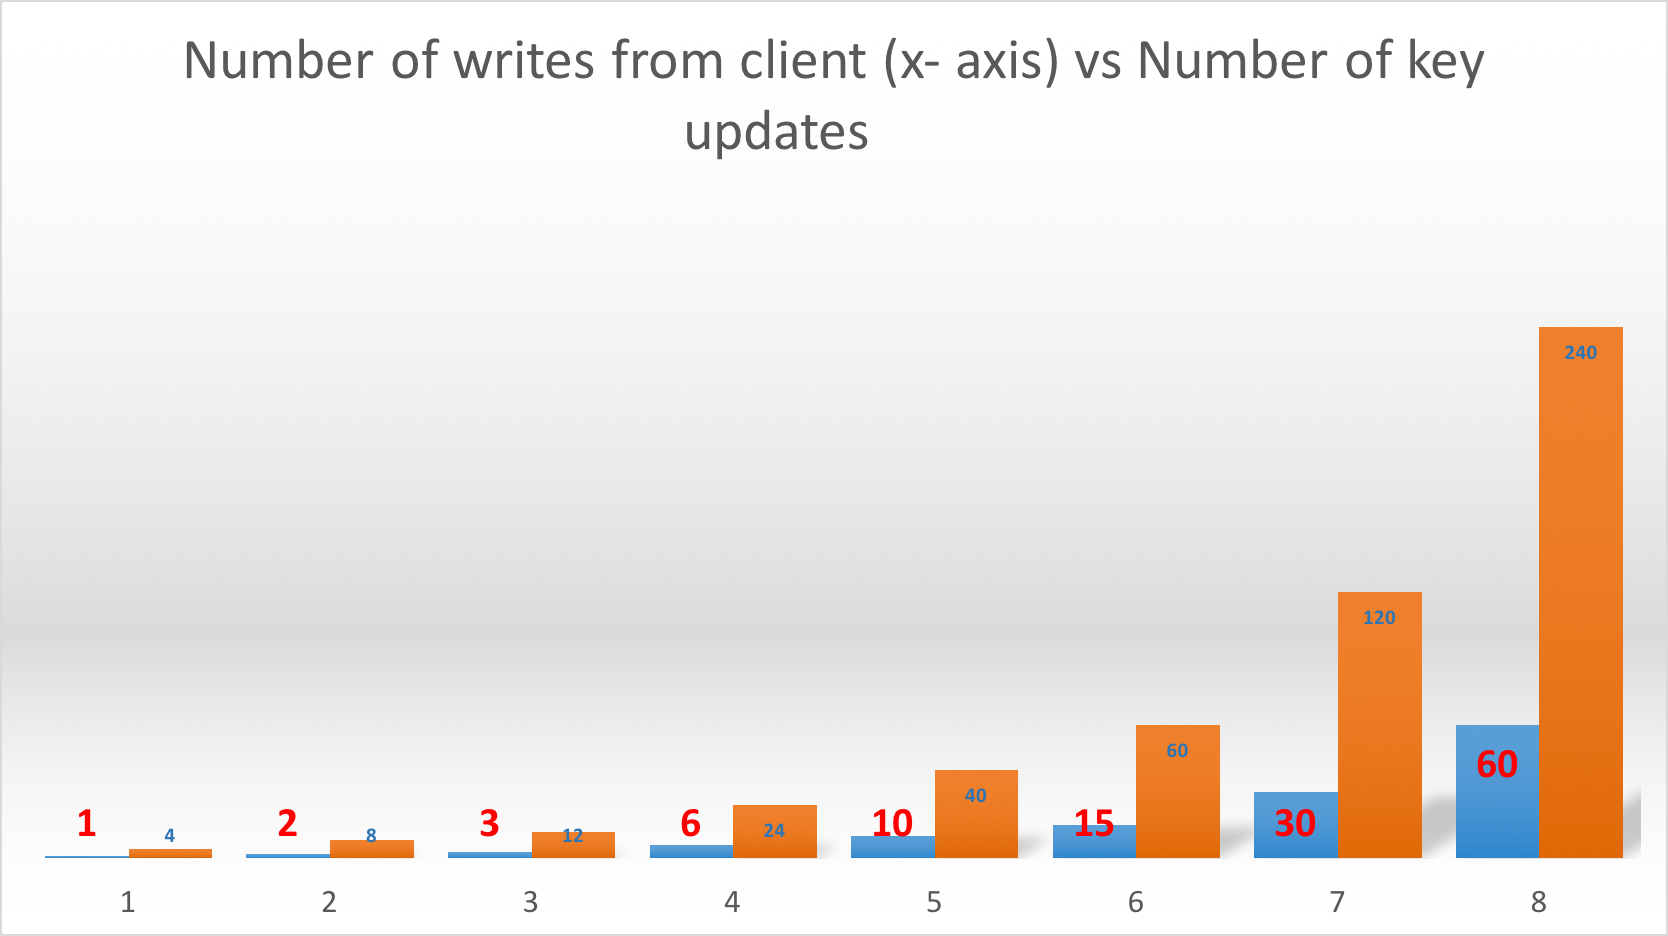
\includegraphics[width=\textwidth]{Plot1}
    \caption{ Theoretical estimate for simple key, value pair distributed system without our solution.}
    \label{fig:8}
\end{figure}

\begin{figure}[!htbp]
    \centering
    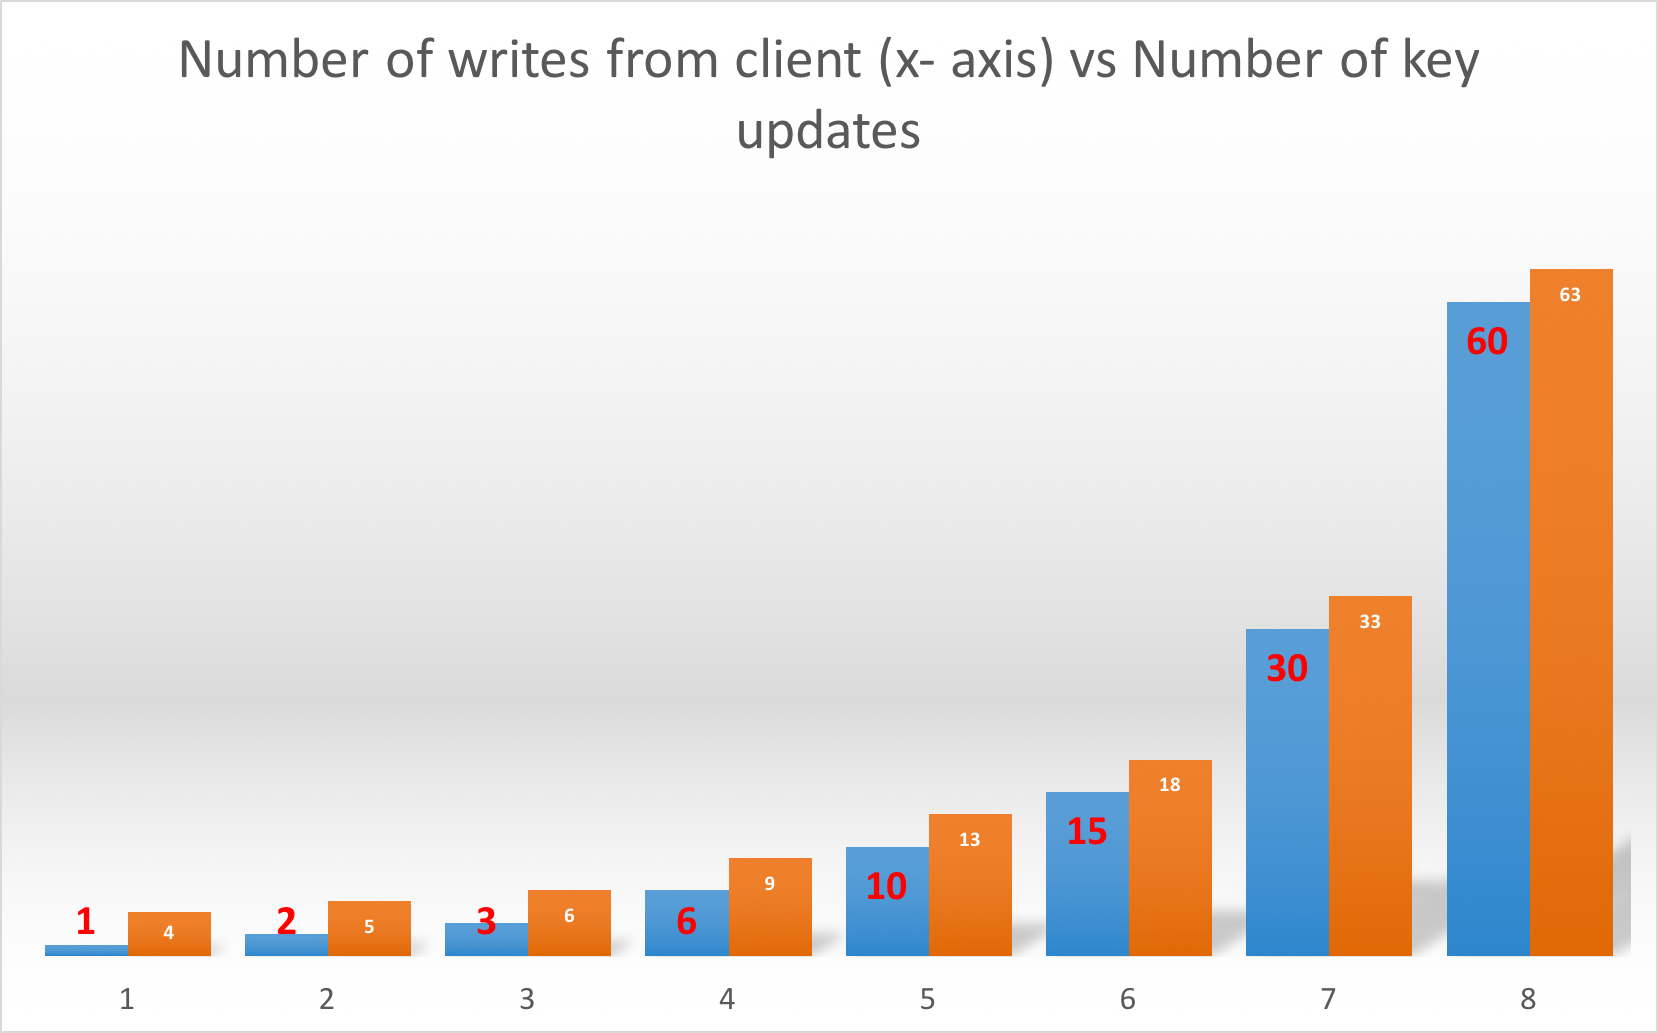
\includegraphics[width=\textwidth]{Plot2}
    \caption{Theoretical estimate for simple key, value pair distributed system with our solution of logging.}
    \label{fig:9}
\end{figure}

Similarly for theoretical analysis lets consider we have the logging mechanism where we have same 4 replication sites. Instead of writing all the writes immediately, the writes are delayed and replicated after 30 seconds. So theoritcally we will be writing only once for each of the key-value update until 30 seconds. Lets assume we will have around 60 writes during 30 seconds, in this scenario there will be only 60 writes to the main replicator and plus 3 for other replictors, which totalls to 63 writes instead of 240 writes. Here we are assuming that we will have 60 update to the same key-value. So we are saving {240 - 63 = 177} writes.

%Once the data is available at one of the replicas instead instantly sending the updates to all the replicas we will accumulated the writes in the log we will wait for 30 second timer and later update the data to all the replicas, by this we were able to save approximately 20 key updates to 3 of the replicas, so we were able to save 60 writes to the flash storage. After 20 key updates our 30 second timer was done and we have to send all the writes accumulated so when we had the 30 key updates we updated all the accumulated key writes to all the replicas. So we are seeing that 120 key update in our solution too in figure 5.



%\newpage
\section{Practical Results}

To implement logging solution as discussed in implementation, we created a timer mechanism in which captured all the writes in the log and wait for specified interval of time say 30 seconds. (This can be tuned as per the requirement and for the remainder of the example we will consider timer of 30 seconds.)
%\begin{figure}[!htbp]
 %   \centering
 %   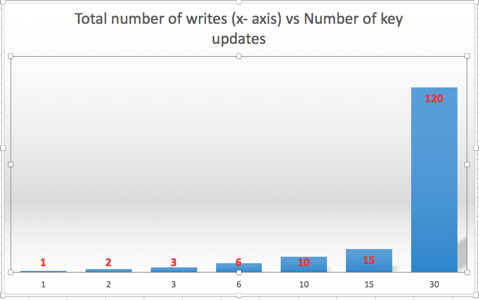
\includegraphics[width=\textwidth]{Figure5}
  %  \caption{Graph for simple key, value pair distributed system with our solution of logging.}
%    \label{fig:9}
%\end{figure}

Practically with our solution we were able to observe the below comparison and there is difference in the theoretical and the practical values. This is because we are using a random number gnerator for load generation and also the timer will not be synced with all the 4 sites.

Figure \ref{fig:10} and \ref{fig:11} are the comparison of total number of writes actually generated at the clients to the total number of writes done at the replicas without and with our solution respectively.

\begin{figure}[!htbp]
    \centering
    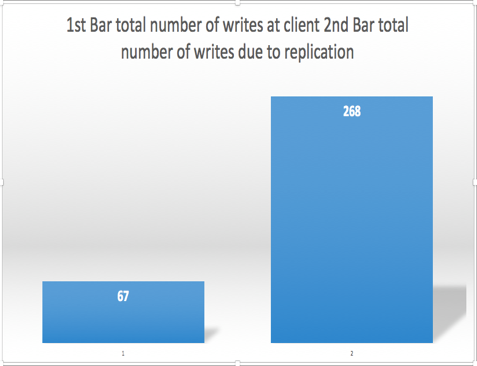
\includegraphics[width=\textwidth]{Figure6}
    \caption{Practical results: Total number of writes from all the clients against the total number of key value updates across replicas without our solution.}
    \label{fig:10}
\end{figure}


The total number of writes for 67 updates with out our solution were 268 writes. Whereas with our solution the number of writes at all the replicas totalled to 157 for the same 67 updates from the client. We can see from this that we were able to save a total of 111 writes, so there was a reduction of 58 percent of writes.

\begin{figure}[!htbp]
    \centering
    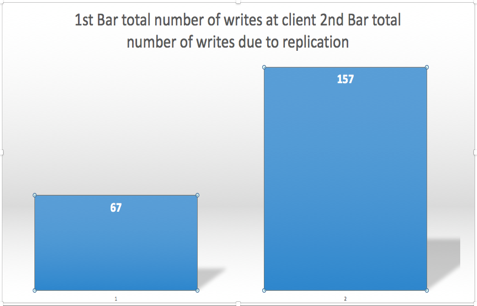
\includegraphics[width=\textwidth]{Figure7}
    \caption{Practical results: Total number of writes from all clients against the total number of key value updates across replicas using the logging solution.}
    \label{fig:11}
\end{figure}

Complete project code is available under: \href{https://github.com/Narendrakumarg1728/write_reduction_in_Distributed_replicas}{GIT HUB link}

\newpage